\section{Пучки прямых, связки и простейшие поверхности}

Этот и следующий разделы расширяют предыдущие: те же средства модели~--- форма абсолюта, полюсы, симметрии~--- применяются к пучкам прямых и их траекториям, а затем к пространству.

\subsection{Нормированные координаты}

Однородные координаты точки определены с точностью до множителя. Для π-точки $k$ выберем представителя
\begin{equation}\label{eq:norm}
X=\frac{(1,k)}{\sqrt{1-|k|^2}},\qquad \sk{X}{X}=-1,\quad x_0>0,
\end{equation}
и назовём его \emph{нормированным вектором} точки. Для внешней точки $P$ (полюса прямой) нормированным будем называть представителя с $\sk{P}{P}=1$. В нормированных координатах формулы раздела~1 упрощаются: по предложению~\ref{prop:ch} $\ch d(X,Y)=-\sk{X}{Y}$, а расстояние от точки $X$ до прямой с нормированным полюсом $P$ равно
\begin{equation}\label{eq:do-pryamoy}
\sh d=|\sk{X}{P}|.
\end{equation}
Для доказательства переведём прямую π-движением на диаметр $k_2=0$ с полюсом $(0:0:1)$; при $X=(1,x,y)/\sqrt{1-x^2-y^2}$ равенство~\eqref{eq:do-pryamoy} совпадает с~\eqref{eq:do-diametra}, переписанным через $\sh d=\thh d/\sqrt{1-\thh^2 d}$.

Наконец, если точка движется по кривой и $X(t)$~--- её нормированный вектор, то из $\ch d=-\sk{X(t)}{X(t+\Delta t)}$ и равенства $\sk{X}{X}=-1$ получается, что элемент длины кривой равен $ds^2=\sk{dX}{dX}$, а касательные векторы $u$ удовлетворяют условию $\sk{u}{X}=0$. Угол между двумя кривыми в общей точке измеряется формой $\sk{\cdot}{\cdot}$ на их касательных векторах; для прямых это согласуется с предложением~\ref{prop:ugol}.

\subsection{Пучки прямых и их траектории}

\begin{definition}[\!\!{[1]}]
\emph{Пучком пересекающихся прямых} называется множество всех прямых, проходящих через точку (центр пучка). \emph{Пучком параллельных прямых} называется множество всех прямых, параллельных данной прямой в данном направлении. \emph{Пучком расходящихся прямых} называется множество всех прямых, перпендикулярных данной прямой (базе пучка).
\end{definition}

\begin{proposition}\label{prop:puchok}
Каждый пучок совпадает с множеством $B_V$ π-прямых, содержащие которые евклидовы прямые проходят через фиксированную точку $V$ проективной плоскости. Для пучка пересекающихся прямых $V$~--- центр пучка (внутренняя точка), для пучка параллельных~--- общий конец прямых (точка абсолюта), для пучка расходящихся~--- полюс базы (внешняя точка).
\end{proposition}
\begin{proof}
Первое утверждение очевидно, второе следует из теоремы~\ref{thm:parallel-model}, третье~--- из леммы~\ref{lem:polyus}.
\end{proof}

Через любую π-точку $A$, отличную от центра пучка, проходит ровно одна прямая пучка: это прямая $AV$. Точку $A$ называют \emph{обыкновенной}, если она не является центром пучка и не лежит на базе~[1].

\begin{definition}[\!\!{[1]}]
\emph{Траекторией} обыкновенной точки $A$ относительно пучка называется множество точек, симметричных $A$ относительно прямых пучка.
\end{definition}

\begin{theorem}\label{thm:traektoriya}
Пусть пучок задан точкой $V$ (с фиксированным представителем), $A$~--- его обыкновенная точка. Траектория точки $A$ есть множество π-точек, нормированные векторы которых удовлетворяют условию
\[
\sk{X}{V}=\sk{A}{V}.
\]
\end{theorem}
\begin{proof}
Пусть $X=\sigma_\ell(A)$, где $\ell$~--- прямая пучка с полюсом $P$. Так как $V$ лежит на $\ell$, то $\sk{V}{P}=0$ и по формуле~\eqref{eq:otrazhenie} $\sigma_\ell(V)=V$. Симметрия сохраняет форму абсолюта и переводит нормированные векторы в нормированные: она непрерывна и оставляет на месте точки прямой $\ell$. Поэтому $\sk{X}{V}=\sk{\sigma_\ell A}{\sigma_\ell V}=\sk{A}{V}$.

Обратно, пусть $\sk{B}{V}=\sk{A}{V}$ и $B\ne A$. Положим $m=A-B$. Тогда
\[
\sk{m}{m}=-2-2\sk{A}{B}=2\bigl(\ch d(A,B)-1\bigr)>0,
\]
то есть $m$~--- внешняя точка, и её поляра $\ell$ является π-прямой. Так как $\sk{A}{m}=-1-\sk{A}{B}=\tfrac12\sk{m}{m}$, по формуле~\eqref{eq:otrazhenie}
\[
\sigma_\ell(A)=A-\frac{2\sk{A}{m}}{\sk{m}{m}}\,m=A-m=B.
\]
Наконец, $\sk{m}{V}=\sk{A}{V}-\sk{B}{V}=0$, то есть $V$ лежит на поляре $\ell$ точки $m$, и прямая $\ell$ принадлежит пучку. Точка $B=A$ получается симметрией относительно прямой пучка, проходящей через $A$.
\end{proof}

Прямая $\ell$ из доказательства~--- серединный перпендикуляр к отрезку $AB$, а её полюс~--- точка $A-B$. Три типа пучков различаются только положением точки $V$, и разбирать их отдельно не понадобилось.

\begin{corollary}\label{cor:traektorii}
Траектория относительно пучка пересекающихся прямых~--- окружность с центром $V$; относительно пучка расходящихся прямых~--- эквидистанта с базой, полярной точке $V$ (по формуле~\eqref{eq:do-pryamoy}); относительно пучка параллельных прямых~--- кривая, которая называется \emph{орициклом}.
\end{corollary}

Подставляя~\eqref{eq:norm} в условие $\sk{X}{V}=c$, где $V=(v_0,\bar v)$, получаем уравнение траектории в координатах круга:
\begin{equation}\label{eq:klein-traektoriya}
(k\cdot\bar v-v_0)^2=c^2\,(1-|k|^2).
\end{equation}
Это кривая второго порядка, и при всех трёх типах пучков она изображается эллипсом или его дугой. Для окружности с центром $q$ и радиусом $\rho$ уравнение имеет вид $(1-k\cdot q)^2=\ch^2\rho\,(1-|q|^2)(1-|k|^2)$; для орицикла с концом $\omega$ на абсолюте~--- $(1-k\cdot\omega)^2=c^2(1-|k|^2)$; для эквидистанты к хорде $k\cdot e=\sigma$ ($|e|=1$, $|\sigma|<1$)~--- $(k\cdot e-\sigma)^2=\sh^2h\,(1-\sigma^2)(1-|k|^2)$. Орицикл касается абсолюта в точке $\omega$, эквидистанта подходит к абсолюту в концах базы, окружность лежит строго внутри круга (рисунок~\ref{fig:puchki}).

\begin{figure}[H]
\centering
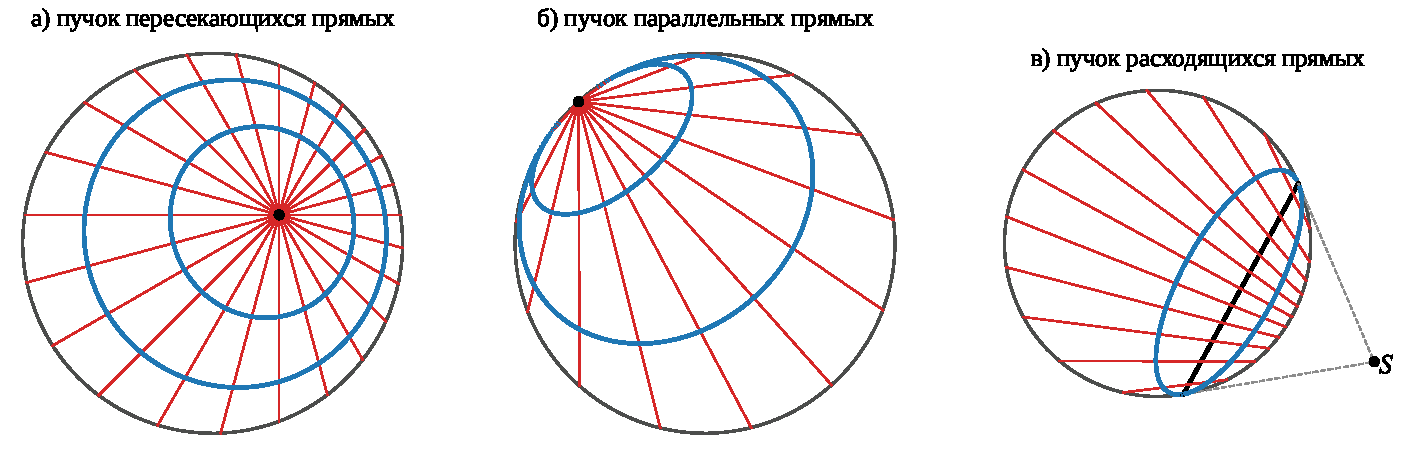
\includegraphics[width=\textwidth]{fig/puchki.pdf}
\caption{Пучки прямых (красные хорды) и их траектории (синие кривые). В случае в) продолжения хорд пучка проходят через полюс $S$ базы (чёрная хорда), синие кривые~--- эквидистанты по обе стороны от базы}
\label{fig:puchki}
\end{figure}

\subsection{Пространство Лобачевского в модели}

Модель пространства устроена так же, как модель плоскости. Абсолютом служит единичная сфера, π-точками~--- внутренние точки шара, π-прямыми~--- хорды, π-плоскостями~--- сечения шара евклидовыми плоскостями, которые его пересекают. Форма абсолюта в однородных координатах $(x_0:x_1:x_2:x_3)$ имеет вид $\sk{X}{Y}=-x_0y_0+x_1y_1+x_2y_2+x_3y_3$. Каждая π-плоскость есть поляра внешней точки, своего полюса; формулы~\eqref{eq:ch}, \eqref{eq:otrazhenie}, \eqref{eq:norm} и~\eqref{eq:do-pryamoy} сохраняются, только $\sigma$ теперь~--- симметрия относительно плоскости, а~\eqref{eq:do-pryamoy} даёт расстояние до плоскости. Повторяя доказательство леммы~\ref{lem:polyus}, получаем: \emph{прямая перпендикулярна плоскости тогда и только тогда, когда продолжение хорды проходит через полюс плоскости}. Проходить через центр шара π-плоскость не обязана.

Две прямые пространства, не лежащие в одной плоскости, называются \emph{скрещивающимися}. Прямые одной плоскости пересекаются, параллельны или расходятся (раздел~2). Расходящиеся и скрещивающиеся прямые имеют единственный общий перпендикуляр~[1]. Две плоскости с нормированными полюсами $P_1$, $P_2$ пересекаются по прямой, если $|\sk{P_1}{P_2}|<1$, параллельны (имеют одну общую точку абсолюта), если $|\sk{P_1}{P_2}|=1$, и расходятся, если $|\sk{P_1}{P_2}|>1$; в последнем случае прямая $P_1P_2$ даёт их единственный общий перпендикуляр. Доказательство повторяет рассуждения п.~2.3.

\subsection{Связки прямых и пучки плоскостей}

\begin{definition}[\!\!{[1]}]
\emph{Связкой пересекающихся прямых} называется множество всех прямых, проходящих через точку $O$. \emph{Связкой параллельных прямых} называется множество всех прямых, параллельных данной прямой в данном направлении. \emph{Связкой расходящихся прямых} называется множество всех прямых, перпендикулярных данной плоскости (базе связки).
\end{definition}

Третью связку не следует путать с пучком расходящихся прямых: прямые одной плоскости, перпендикулярные одной прямой, образуют пучок, и поверхности, перпендикулярной всем им, в пространстве нет.

\begin{proposition}\label{prop:svyazka}
Каждая связка совпадает с множеством $B_V$ π-прямых, продолжения которых проходят через фиксированную точку $V$: внутреннюю для связки пересекающихся прямых, лежащую на абсолюте для связки параллельных и внешнюю (полюс базы) для связки расходящихся.
\end{proposition}
\begin{proof}
Первые два случая разбираются так же, как в предложении~\ref{prop:puchok}, третий следует из описания перпендикуляра к плоскости.
\end{proof}

\emph{Пучок плоскостей}~--- это множество π-плоскостей, содержащих одну евклидову прямую $u$. Если $u$ пересекает шар, это все плоскости, проходящие через π-прямую. Если $u$ касается абсолюта в точке $\omega$, все плоскости пучка проходят через $\omega$ и попарно параллельны. Если $u$ лежит вне шара, все плоскости пучка перпендикулярны одной π-прямой, полярной прямой $u$: плоскость с полюсом $P$ перпендикулярна прямой тогда и только тогда, когда продолжение этой прямой проходит через $P$.

\subsection{Простейшие поверхности как траектории связок}

Плоскость, проходящую через точку $V$, назовём \emph{плоскостью связки} $B_V$. Каждая плоскость связки состоит из прямых связки.

\begin{theorem}\label{thm:svyazka}
Пусть связка задана точкой $V$, $c$~--- число, и множество
\[
S=\{X:\ \sk{X}{X}=-1,\ x_0>0,\ \sk{X}{V}=c\}
\]
непусто и не содержит центра связки. Тогда:
\begin{enumerate}
  \item через каждую точку $X\in S$ проходит ровно одна прямая связки, и она перпендикулярна поверхности $S$;
  \item связная поверхность, перпендикулярная всем прямым связки, которые она пересекает, целиком лежит на одной из поверхностей $S$;
  \item $S$~--- множество точек, симметричных фиксированной точке $A\in S$ относительно плоскостей связки;
  \item пересечение $S$ с любой плоскостью связки~--- траектория соответствующего пучка прямых в этой плоскости.
\end{enumerate}
\end{theorem}
\begin{proof}
1. Касательные векторы $u$ к поверхности $S$ в точке $X$ удовлетворяют условиям $\sk{u}{X}=0$ и $\sk{u}{V}=0$. Прямая связки через $X$ лежит в евклидовой плоскости, натянутой на векторы $X$ и $V$ (они не пропорциональны, так как $X$ не центр). Её касательный вектор в точке $X$ получается из $V$ вычитанием составляющей вдоль $X$:
\[
w=V+\sk{X}{V}\,X,\qquad \sk{w}{X}=\sk{X}{V}-\sk{X}{V}=0.
\]
Для любого касательного вектора $u$ к $S$ имеем $\sk{u}{w}=\sk{u}{V}+\sk{X}{V}\sk{u}{X}=0$, то есть прямая перпендикулярна $S$.

2. Вектор $w$ направлен по градиенту функции $f(X)=\sk{X}{V}$ на множестве нормированных векторов. Если поверхность перпендикулярна всем прямым связки, производная $f$ вдоль неё равна нулю, и на связной поверхности $f$ постоянна.

3. Для плоскости связки с полюсом $P$ выполнено $\sk{V}{P}=0$, симметрия оставляет $V$ на месте и сохраняет $f$. Обратное включение доказывается теми же выкладками с вектором $m=A-B$, что и в теореме~\ref{thm:traektoriya}.

4. На плоскости связки $\Sigma$ форма абсолюта индуцирует форму абсолюта этой плоскости, точка $V$ задаёт в ней пучок, и $S\cap\Sigma$ описывается тем же уравнением $\sk{X}{V}=c$. По теореме~\ref{thm:traektoriya} это траектория пучка.
\end{proof}

\begin{corollary}\label{cor:poverhnosti}
\begin{enumerate}
  \item Если $V=O$~--- внутренняя точка, то $S$ при $c=-\ch\rho$~--- \emph{сфера} с центром $O$ радиуса $\rho$. Её сечение плоскостью, проходящей через центр,~--- окружность того же радиуса.
  \item Если $V=\ell$~--- точка абсолюта, то $S$~--- \emph{орисфера}. Её сечение плоскостью, проходящей через $\ell$,~--- орицикл.
  \item Если $V=P$~--- полюс плоскости $\Pi$, то $S$ при $c=\sh h$~--- \emph{эквидистантная поверхность}, множество точек одной стороны от $\Pi$, удалённых от неё на $h$. Её сечение плоскостью, перпендикулярной $\Pi$,~--- эквидистанта.
\end{enumerate}
\end{corollary}

Утверждения о том, что сфера, орисфера и эквидистантная поверхность ортогональны соответствующим связкам, получают одно общее доказательство.

\subsection{Изображение поверхностей в модели}

Подставим $X=(1,k)/\sqrt{1-|k|^2}$, $k\in\R^3$, $|k|<1$, в уравнение $\sk{X}{V}=c$:
\begin{equation}\label{eq:klein-poverhnost}
(k\cdot\bar v-v_0)^2=c^2\,(1-|k|^2),\qquad V=(v_0,\bar v).
\end{equation}
Это поверхность второго порядка, квадратичная часть $(k\cdot\bar v)^2+c^2|k|^2$ положительно определена, поэтому все три поверхности изображаются эллипсоидами или их частями.

\begin{remark}
Уравнение~\eqref{eq:klein-poverhnost} имеет вид $F_1^2-c^2F_2=0$, где $F_2=0$~--- уравнение абсолюта, а $F_1=0$~--- уравнение плоскости, полярной точке $V$~[7]. Значит, все три поверхности принадлежат пучку квадрик, порождённому абсолютом и сдвоенной полярной плоскостью точки $V$, и касаются абсолюта вдоль сечения этой плоскостью. Для сферы полярная плоскость центра лежит вне шара, и касание мнимое; для орисферы это касательная плоскость в точке $\ell$; для эквидистантной поверхности это сама база $\Pi$, и поверхность подходит к абсолюту по окружности, по которой его пересекает база.
\end{remark}

\textbf{Сфера.} Пусть центр изображается точкой $q$, $a=|q|<1$, радиус равен $\rho$, $C=\ch^2\rho$. Уравнение~\eqref{eq:klein-poverhnost} принимает вид $(1-k\cdot q)^2=C(1-a^2)(1-|k|^2)$. Направим ось $z$ вдоль $q$ и обозначим через $y$ расстояние от точки до этой оси. Тогда $(1-az)^2=C(1-a^2)(1-z^2-y^2)$. Положим $B=a^2+C(1-a^2)$. Выделяя полный квадрат по $z$, получаем
\[
B\Bigl(z-\frac aB\Bigr)^2+C(1-a^2)\,y^2=\frac{C(C-1)(1-a^2)^2}{B}.
\]
Следовательно, сфера изображается эллипсоидом вращения с осью вдоль $q$, евклидовым центром $q/B$ и полуосями
\begin{equation}\label{eq:sfera-poluosi}
r_\perp=\sqrt{\frac{(1-a^2)(C-1)}{B}},\qquad r_\parallel=\frac{(1-a^2)\sqrt{C(C-1)}}{B}.
\end{equation}
Евклидов центр эллипсоида $q/B$ совпадает с изображением центра сферы только при $q=0$. При $a=0{,}6$ и $\rho=1$ получаем $B\approx1{,}884$, евклидов центр на расстоянии $0{,}318$ от центра шара, $r_\perp\approx0{,}685$, $r_\parallel\approx0{,}616$. При малом $\rho$ имеем $C\approx1$ и $B\approx1$, и евклидов центр почти совпадает с $q$. С ростом радиуса он всё дальше отходит от $q$ к центру шара (рисунок~\ref{fig:sravnenie}).

\begin{figure}[H]
\centering
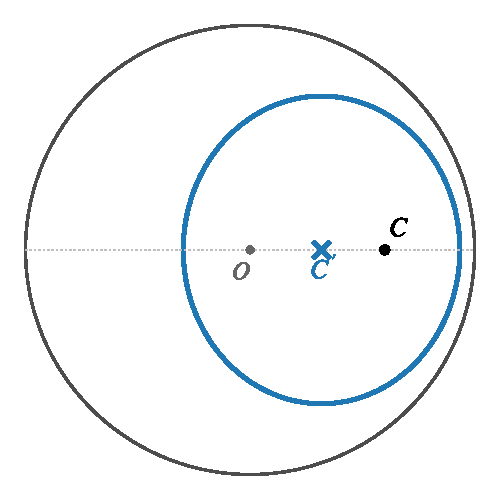
\includegraphics[width=0.46\textwidth]{fig/sravnenie.pdf}
\caption{Сечение сферы с центром $C$ ($a=0{,}6$, $\rho=1$) плоскостью, проходящей через центр шара $O$: эллипс, изображение центра $C$ и евклидов центр эллипса $C'$}
\label{fig:sravnenie}
\end{figure}

\textbf{Орисфера.} Для $\ell=(1,\omega)$, $|\omega|=1$, уравнение~\eqref{eq:klein-poverhnost} даёт $(1-k\cdot\omega)^2=c^2(1-|k|^2)$. Направим ось $z$ вдоль $\omega$; тогда $(1-z)^2=c^2(1-z^2-y^2)$, и после выделения полного квадрата
\[
c^2y^2+(1+c^2)\Bigl(z-\frac1{1+c^2}\Bigr)^2=\frac{c^4}{1+c^2}.
\]
При $r=c/\sqrt{1+c^2}$ это эллипсоид вращения с полуосями $r$ поперёк оси и $r^2$ вдоль неё и с центром $(1-r^2)\omega$, касающийся абсолюта в точке $\omega$. Для сравнения: в модели Пуанкаре орисфера изображается евклидовой сферой, касающейся абсолюта в той же точке.

\textbf{Эквидистантная поверхность} к плоскости $k\cdot e=\sigma$ ($|e|=1$, $|\sigma|<1$) задаётся уравнением $(k\cdot e-\sigma)^2=\sh^2h\,(1-\sigma^2)(1-|k|^2)$. При $\sigma=0$, $e=(0,0,1)$ получаем $z=\pm\thh h\,\sqrt{1-x^2-y^2}$, пространственный аналог предложения~\ref{prop:ekvidistanta}.

На рисунке~\ref{fig:poverhnosti} сфера и орисфера изображены похожими эллипсоидами, и различаются они положением относительно абсолюта. Сфера лежит строго внутри шара: её эллипсоид нигде не касается граничной сферы, а прямые связки сходятся в центре $O$ внутри шара. Орисфера касается абсолюта в точке $\omega$, и все прямые её связки выходят из этой точки, то есть попарно параллельны. Если уводить центр сферы, проходящей через фиксированную точку, к точке $\omega$, сферы стремятся к орисфере; в интерактивной модели этому посвящена сцена «От сферы к орисфере». Эквидистантная поверхность подходит к абсолюту по целой окружности, по той, по которой его пересекает база.

\begin{figure}[H]
\centering
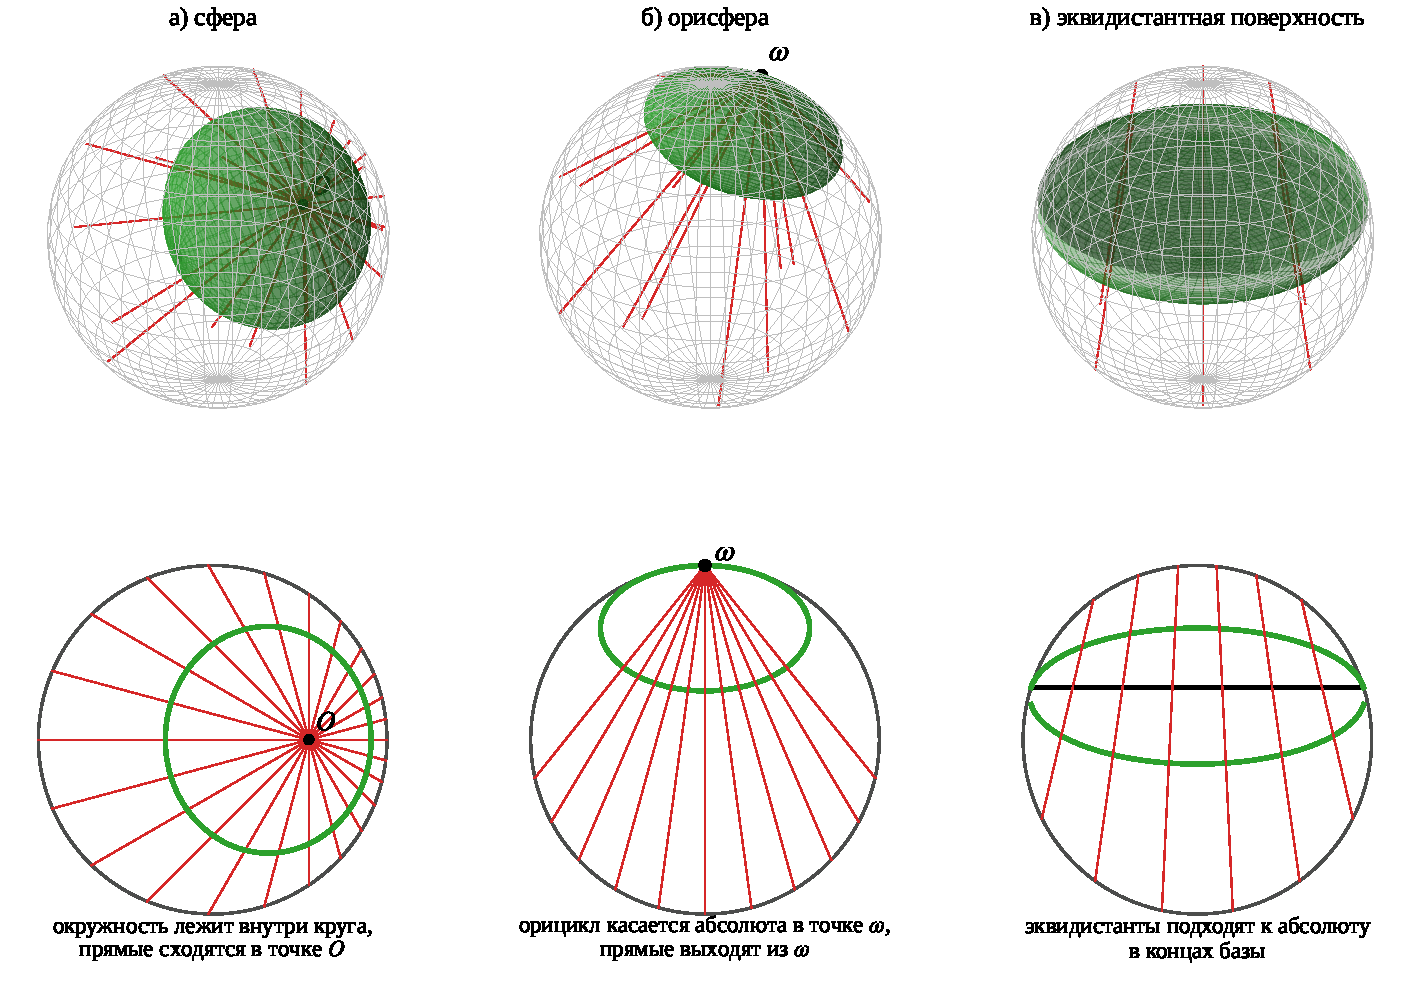
\includegraphics[width=\textwidth]{fig/poverhnosti.pdf}
\caption{Верхний ряд: а) сфера с центром $O$ и прямые собственной связки; б) орисфера и прямые связки параллельных прямых, выходящие из точки $\omega$ абсолюта; в) эквидистантная поверхность к плоскости $z=0{,}3$ и перпендикуляры к этой плоскости, продолжения которых сходятся в её полюсе. Нижний ряд: сечения тех же поверхностей плоскостью, проходящей через центр шара и ось поверхности}
\label{fig:poverhnosti}
\end{figure}

\subsection{Внутренняя геометрия поверхностей}

\begin{theorem}\label{thm:krivizna}
Внутренняя геометрия сферы радиуса $\rho$~--- геометрия евклидовой сферы радиуса $\sh\rho$, её гауссова кривизна равна $1/\sh^2\rho$. Внутренняя геометрия орисферы евклидова. Внутренняя геометрия эквидистантной поверхности на расстоянии $h$ от базы~--- геометрия плоскости Лобачевского с кривизной $-1/\ch^2h$.
\end{theorem}
\begin{proof}
\emph{Сфера.} Нормированные векторы точек сферы с центром $O$ имеют вид $X=\ch\rho\,O+\sh\rho\,u$, где $u$ пробегает векторы с $\sk{u}{O}=0$ и $\sk{u}{u}=1$. На векторах, ортогональных внутренней точке $O$, форма абсолюта положительно определена, то есть задаёт обычное евклидово скалярное произведение. Так как $dX=\sh\rho\,du$ и $ds^2=\sk{dX}{dX}$, длины на сфере в $\sh\rho$ раз больше длин на единичной евклидовой сфере.

\emph{Эквидистантная поверхность.} Каждую её точку можно записать как $X=\ch h\,Y+\sh h\,P$, где $P$~--- нормированный полюс базы, а $Y=(X-\sh h\,P)/\ch h$ лежит на базе: $\sk{Y}{P}=0$ и $\sk{Y}{Y}=-1$. Так как $dX=\ch h\,dY$, метрика поверхности в $\ch^2h$ раз больше метрики плоскости Лобачевского, и кривизна делится на $\ch^2h$.

\emph{Орисфера.} π-движением можно перевести точку абсолюта в $\ell=(1,0,0,1)$, а орисферу~--- в поверхность $\sk{X}{\ell}=-1$. Она параметризуется так:
\[
X(u)=\Bigl(1+\tfrac{|u|^2}2,\ u_1,\ u_2,\ \tfrac{|u|^2}2\Bigr),\qquad u=(u_1,u_2)\in\R^2.
\]
Проверка: $\sk{X}{X}=-(1+\tfrac{|u|^2}2)^2+|u|^2+\tfrac{|u|^4}4=-1$ и $\sk{X}{\ell}=-1$. Дифференцируя, получаем $dX=(u\cdot du,\ du_1,\ du_2,\ u\cdot du)$ и
\[
\sk{dX}{dX}=-(u\cdot du)^2+du_1^2+du_2^2+(u\cdot du)^2=du_1^2+du_2^2.
\]
Орисфера изометрична евклидовой плоскости.
\end{proof}

Кривизна сферы Лобачевского $1/\sh^2\rho$ меньше кривизны евклидовой сферы того же радиуса $1/\rho^2$, так как $\sh\rho>\rho$: при $\rho=1$ это $0{,}72$ против $1$. Параметризация $X(u)$ показывает и переход к концентрической орисфере. Точка прямой связки, лежащая на орисфере $\sk{X}{\ell}=-c'$, равна $c'X(u)+\tfrac{1-c'^2}{2c'}\,\ell$, поэтому метрика на этой орисфере в тех же координатах $u$ равна $c'^2(du_1^2+du_2^2)$. Если сдвинуться вдоль прямых связки на расстояние $h$ в сторону точки $\ell$, то $c'=e^{-h}$, и все длины уменьшаются в $e^{h}$ раз.
